%31/01 - Modesto
\chapter{Bases de datos de proteínas}
\section{Comparación de estructura y alineamiento}
Para comprender la diversidad y función de las proteínas, es importante comparar sus secuencias y estructuras. Esto ayuda a encontrar patrones comunes y a comprender su diversidad e historia evolutiva. Midiendo y analizando estas similitudes, los científicos pueden clasificar las proteínas y determinar sus relaciones en términos de función y evolución. Este proceso también es crucial en el modelado de proteínas, ya que ayuda a identificar, evaluar y elegir modelos intermedios.

Es esencial aclarar la distinción entre alineamiento y superposición, ya que estos términos se confunden con frecuencia en la literatura. Un \textbf{alineamiento estructural} pretende identificar similitudes y diferencias entre dos estructuras, mientras que la \textbf{superposición de estructuras} muestra las estructuras basándose en criterios específicos, normalmente derivados de un alineamiento estructural previo. Por consiguiente, la superposición trata de minimizar la distancia entre estructuras identificando una transformación que consiga la menor desviación cuadrática media (RMSD) o las máximas equivalencias dentro de un límite RMSD.

La RMSD puede calcularse para cualquier par de moléculas. En el contexto de las proteínas, solemos referirnos a la RMSD de los alfa-carbones. Una alineación superior facilitará una mejor superposición. Por lo tanto, aunque la alineación y la superposición son procesos distintos, la RMSD puede servir como indicador de ambos; cuanto menor sea la RMSD, mejor será la alineación/superposición. Es importante señalar que la RMSD es una medida de distancia real, no una puntuación. Eso implica que sólo podemos obtener la RMSD para los residuos alineados, no para toda la secuencia de cualquiera de las dos proteínas. Por lo tanto, una RMSD de 1 $\AA$ puede indicar una distancia cercana pero, si implica a muy pocos aminoácidos, no sugiere necesariamente una buena similitud. Tanto el valor RMSD como el número de residuos alineados deben tenerse en cuenta para un análisis preciso.

\begin{figure}[h]
\centering
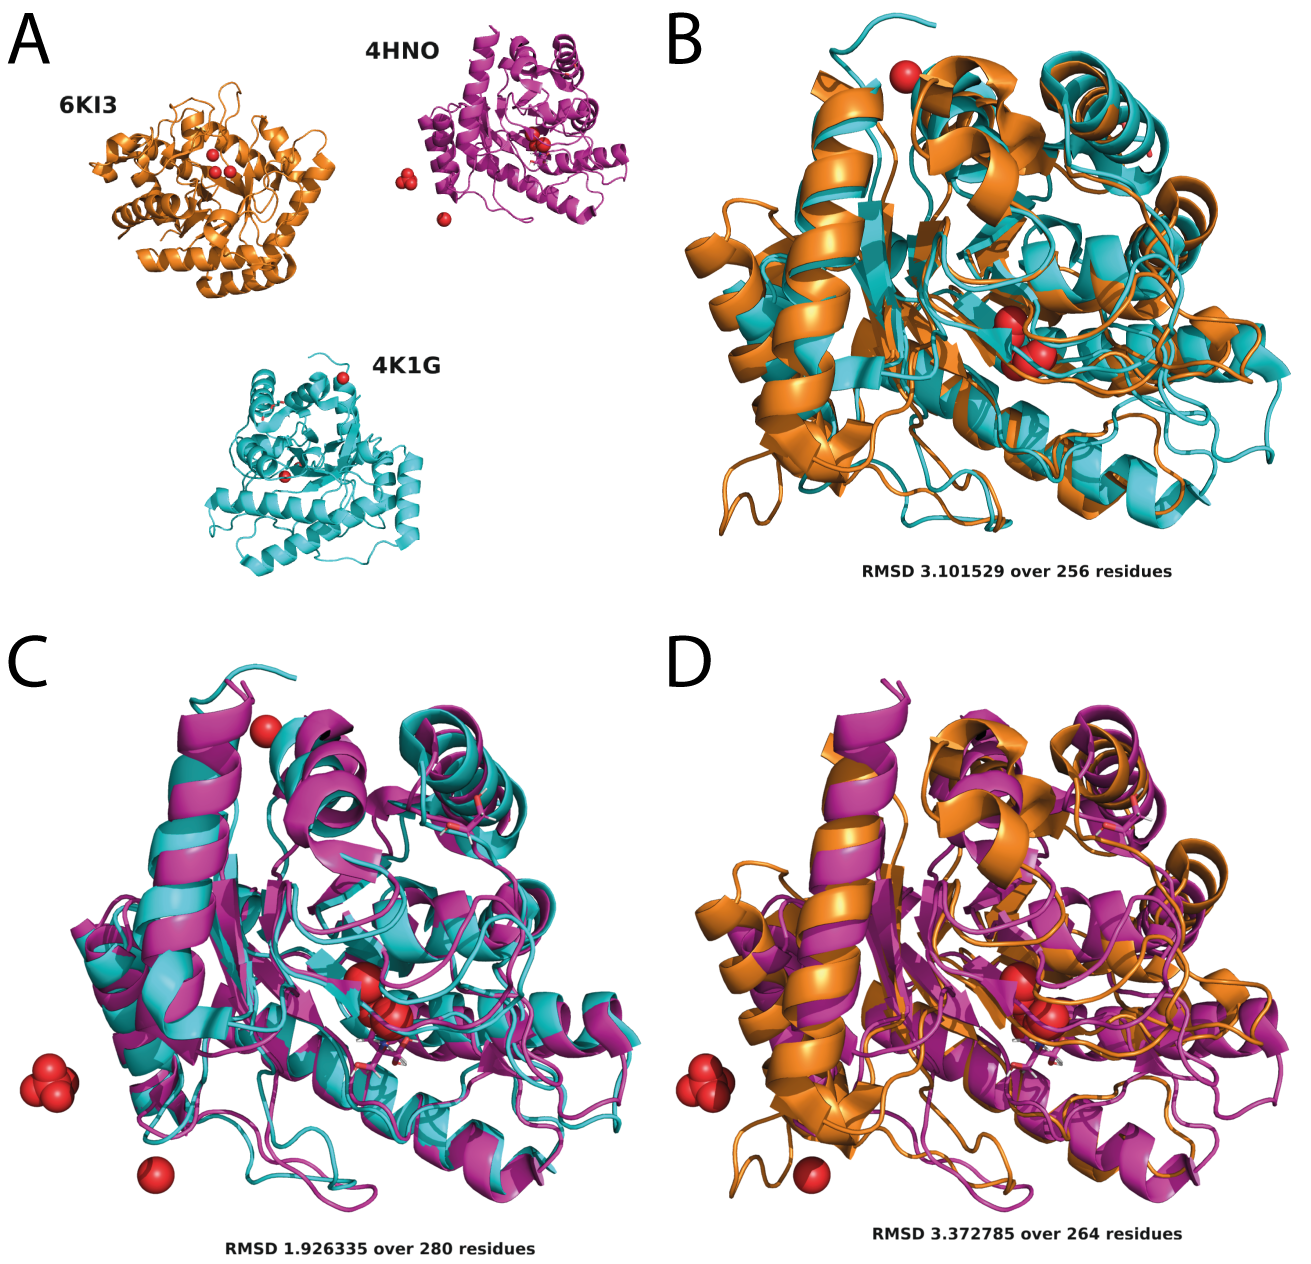
\includegraphics[width = 0.6\textwidth]{figs/rmsd.png}
\end{figure}

Global Distance Test se utiliza en CASP al ser menos sensible a outliers y permite comparar estructuras de secuencias idénticas. Se normaliza el número de residuos que caigan bajo un límite.

\section{Principales bases de datos de proteínas}
La clasificación de secuencias proteicas nos ayuda a comprender la diversidad de las distintas proteínas mediante el examen de sus secuencias, lo que se conoce como el \textbf{espacio de secuencias proteicas} (el concepto matemático de espacio). Por otro lado, la clasificación de las estructuras proteicas consiste en agrupar las proteínas en función de sus relaciones estructurales. Algunas clasificaciones tienen en cuenta la vecindad estructural (continuo estructural), mientras que otras utilizan el concepto de evolución de las proteínas como principal factor de diversificación, lo que da lugar a un \textbf{espacio de estructuras proteicas} discreto en lugar de continuo.

Esta sección no pretende ofrecer una revisión exhaustiva de todas las bases de datos de proteínas. En consecuencia, no cubriremos en detalle la base de datos de proteínas del NCBI, que se utiliza ampliamente para diversos fines y probablemente se mencione en otros cursos. La Base de Datos de Proteínas del NCBI sirve principalmente como repositorio principal de secuencias, con un énfasis mínimo en el análisis de la diversidad y clasificación de proteínas. Esta sección destacará las principales diferencias y aplicaciones de Pfam, Uniprot, Prosite, PDB, SCOP y CATH. 

\begin{figure}[h]
\centering
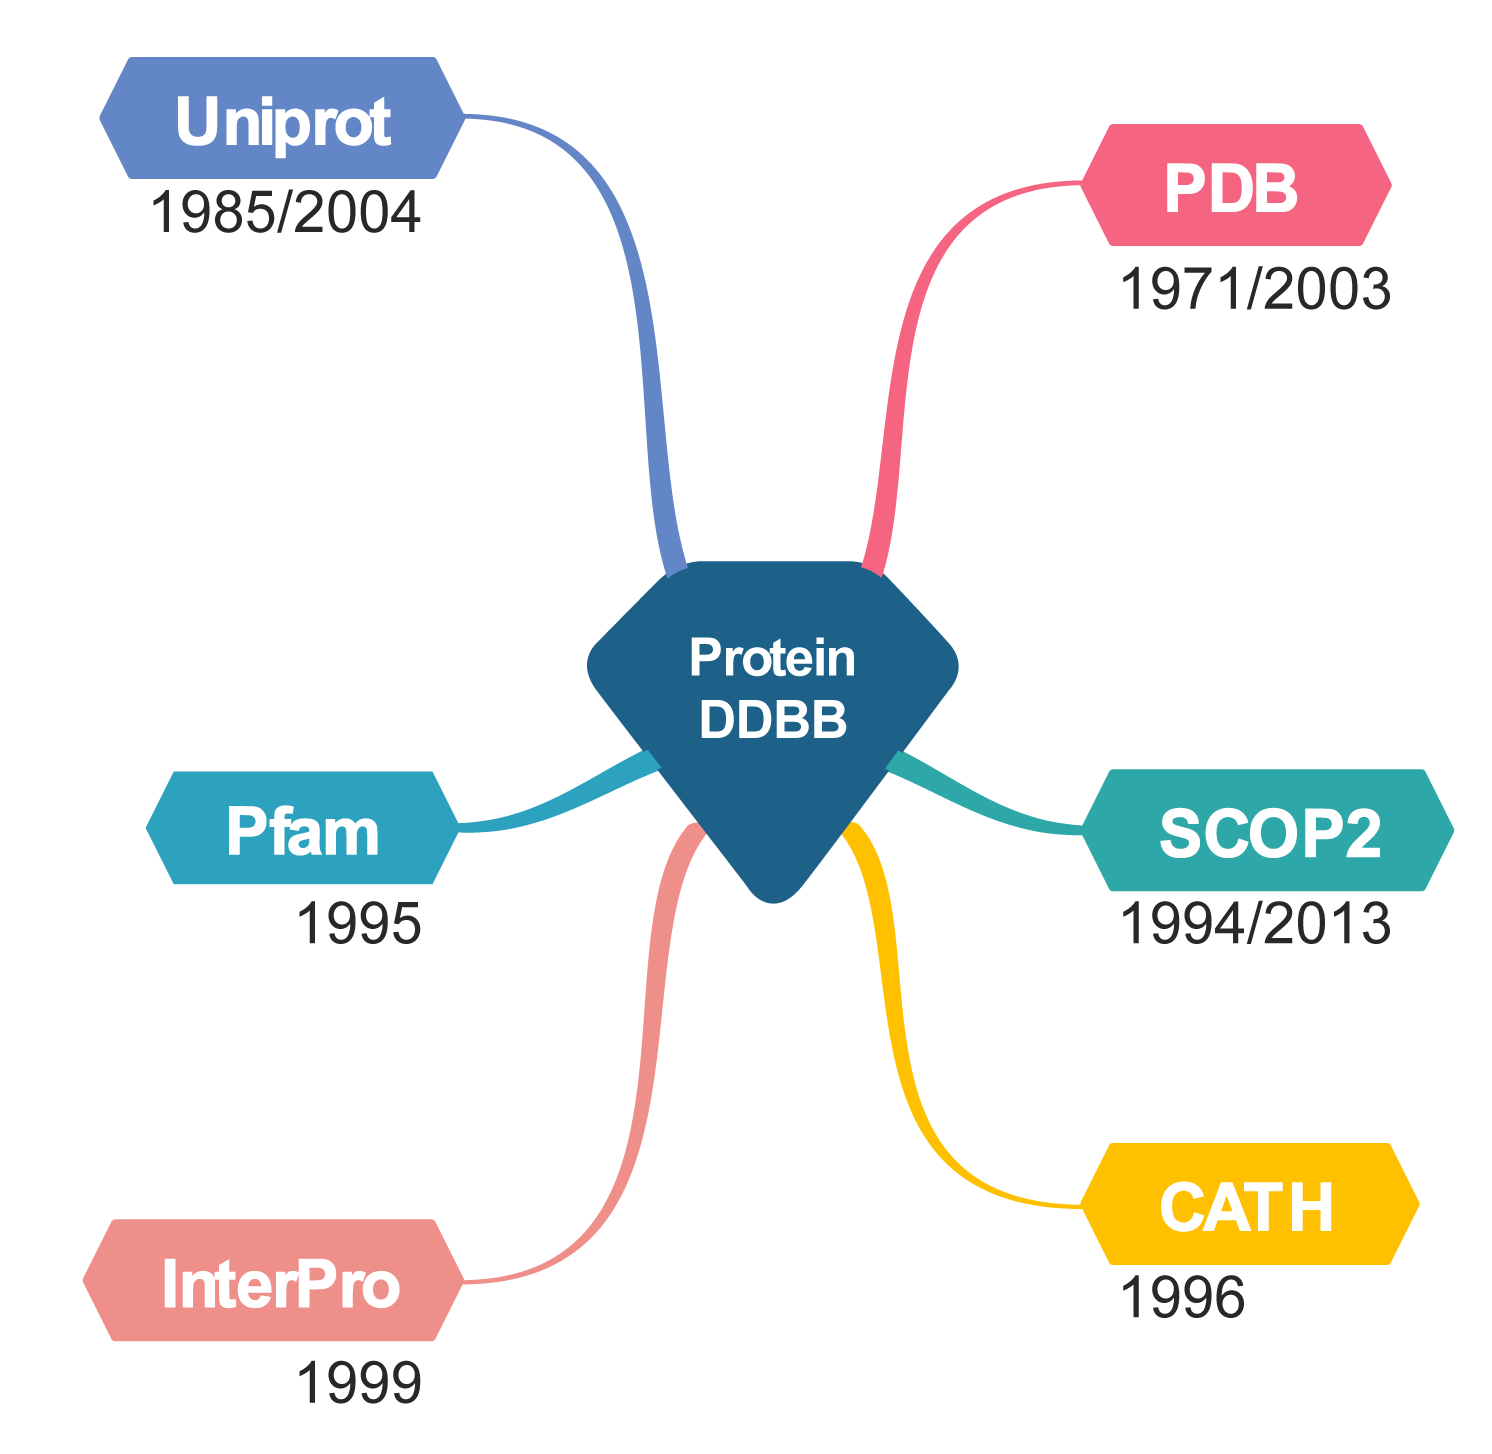
\includegraphics[width = 0.4\textwidth]{figs/ddbb.png}
\end{figure}

En bioinformática, las bases de datos suelen clasificarse en primarias o secundarias. Las \textbf{bases de datos primarias} contienen datos obtenidos experimentalmente, como secuencias de nucleótidos, secuencias de proteínas o estructuras macromoleculares. Es importante señalar que, una vez asignado el número de acceso a una base de datos, los datos de las bases de datos primarias permanecen inalterados y forman parte del registro científico. En cambio, las \textbf{bases de datos secundarias} incluyen datos derivados del análisis de datos primarios. Estas bases de datos suelen utilizar información procedente de numerosas fuentes, incluidas otras bases de datos y la literatura científica. Suelen ser muy complejas e implican una compleja combinación de algoritmos informáticos y/o análisis e interpretación manuales para generar nuevos conocimientos a partir del registro público de la ciencia.

Aunque la distinción entre bases de datos primarias y secundarias se ha vuelto menos clara en los últimos tiempos debido a la integración de datos procedentes de diversas fuentes, aún pueden distinguirse algunas diferencias. Las principales bases de datos primarias para secuencias de proteínas son NCBI Protein y RCSB-PDB para estructuras proteicas. UniProt también alberga una base de datos primaria de secuencias denominada TrEMBL y, desde 2002, incorpora la base de datos PIR-PSD, que reúne los recursos de Protein Information Resource, EMBL y SIB en una única metabase de datos (véase PIR-PSD). Por otra parte, RCSB-PDB es la principal base de datos estructural primaria, mientras que SCOP2 y CATH son bases de datos secundarias notables.

\begin{figure}[h]
\centering
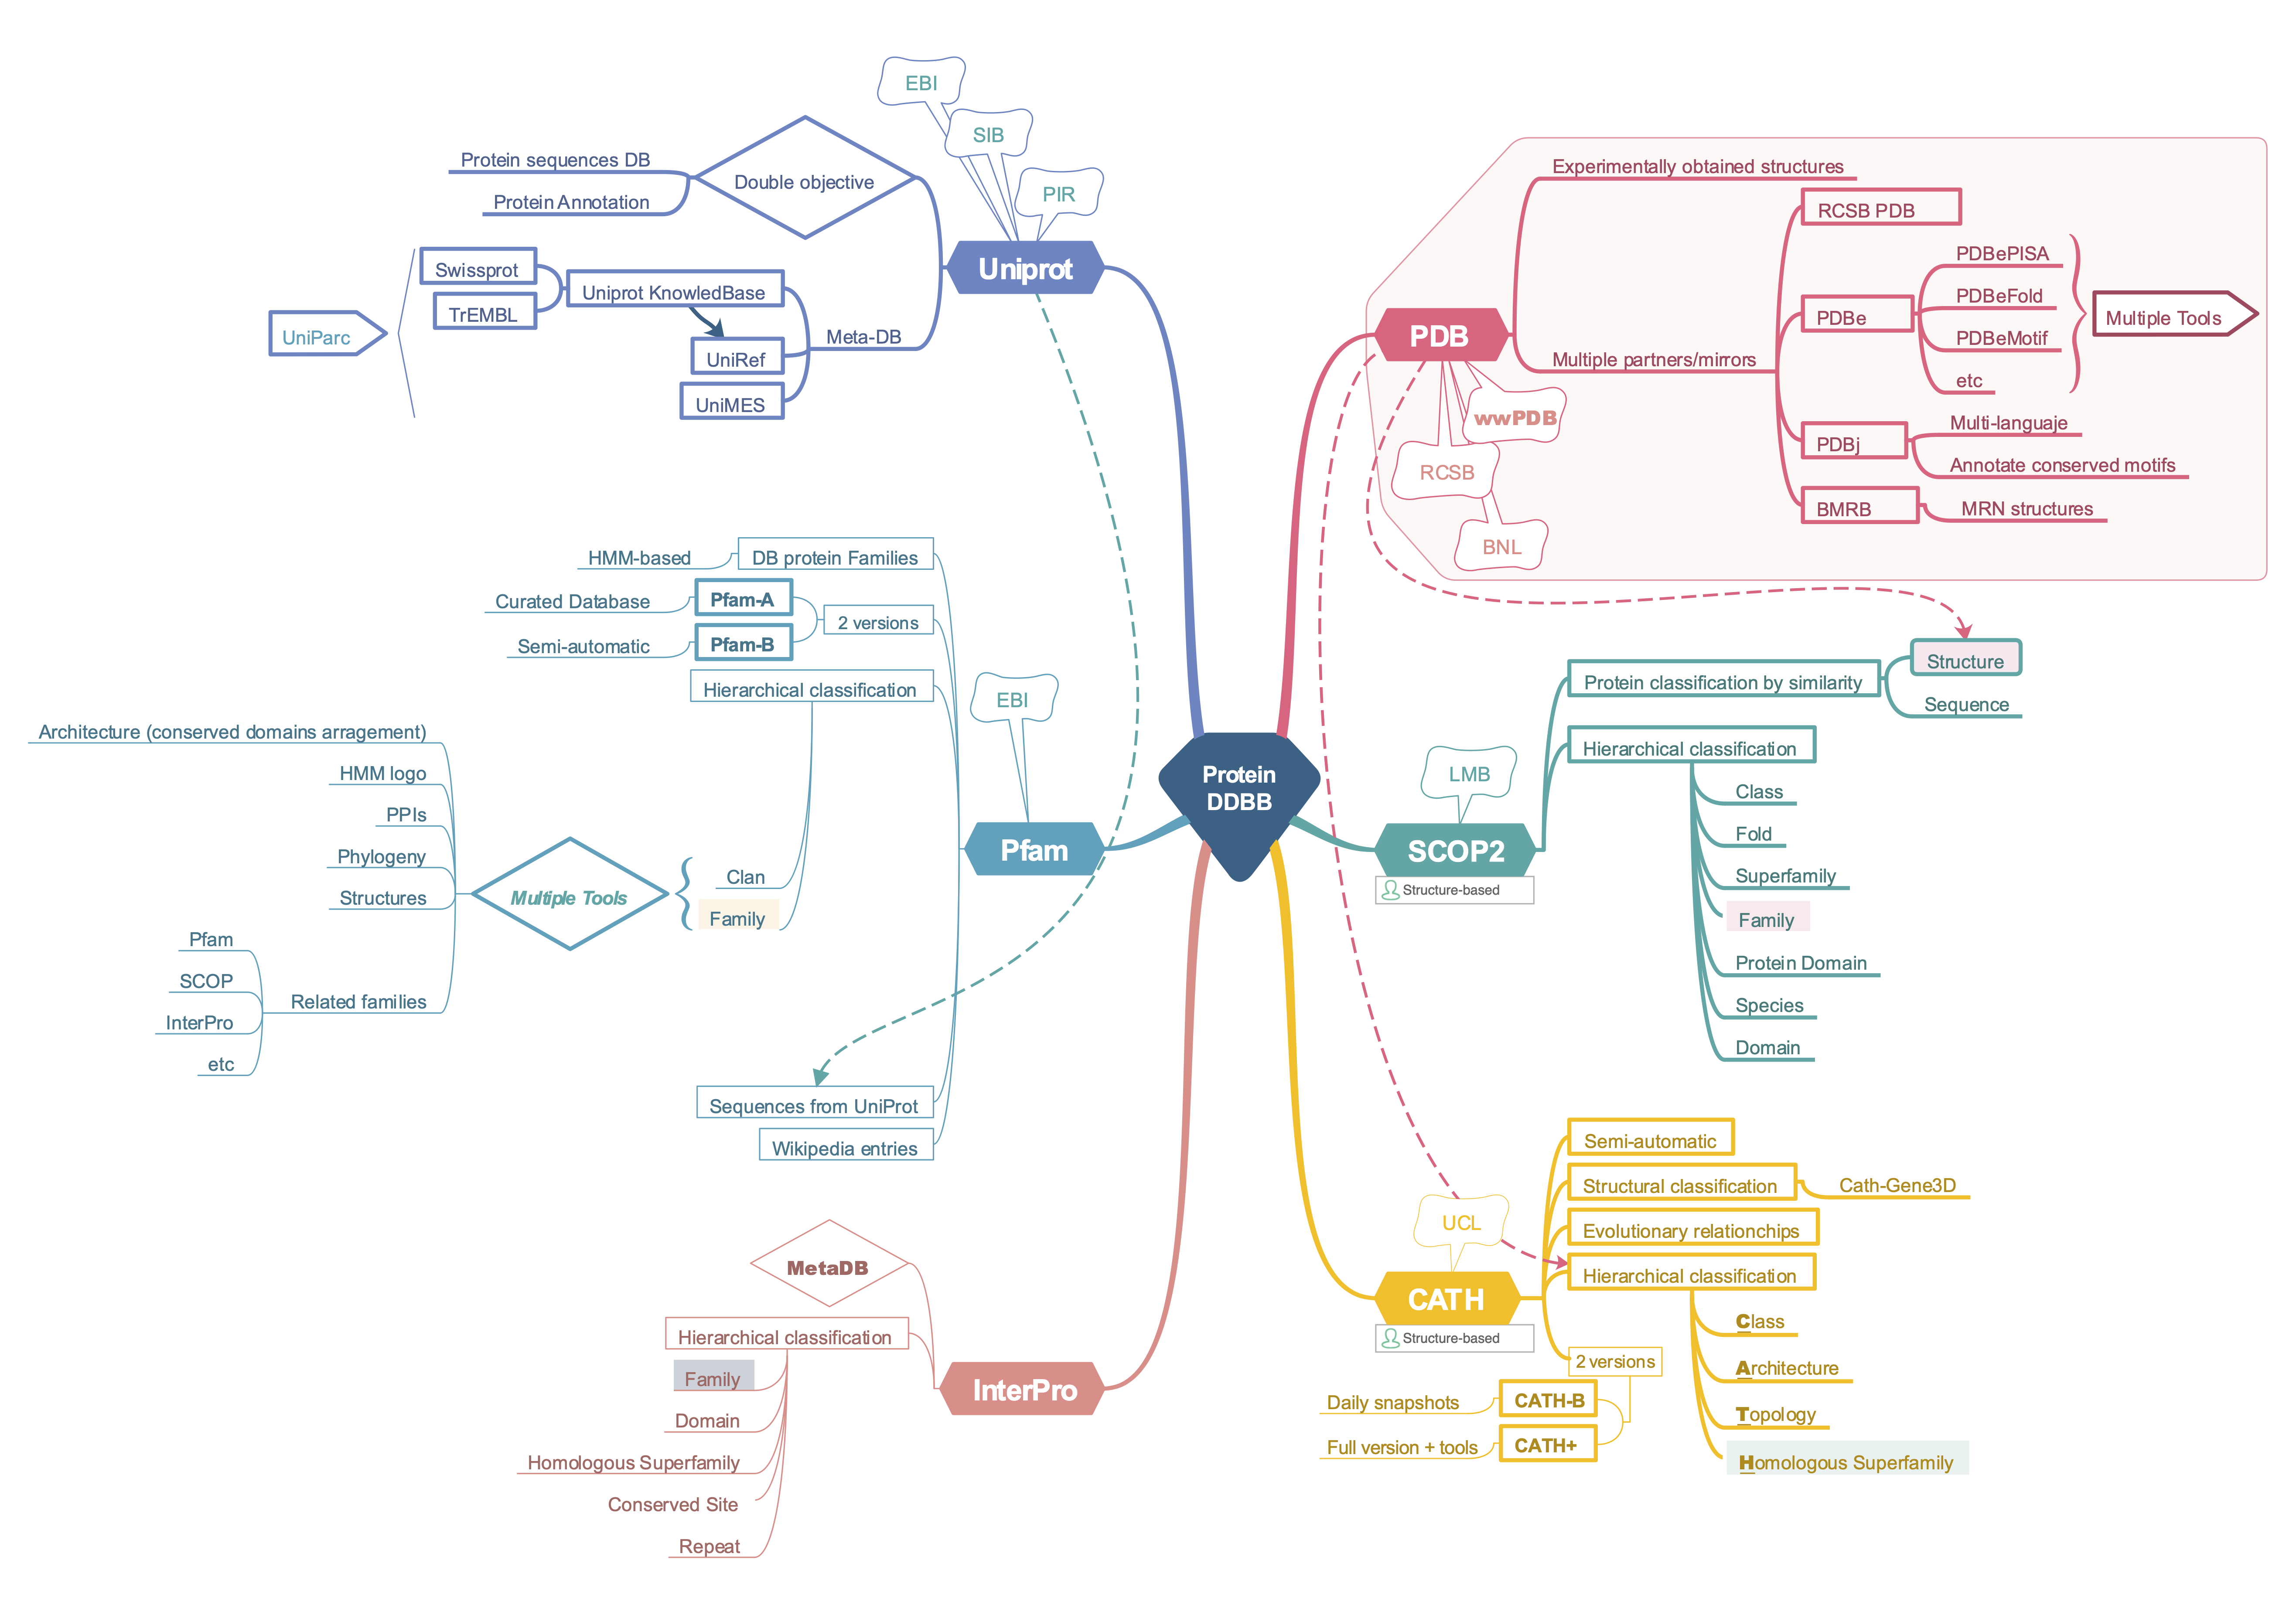
\includegraphics[width = 0.9\textwidth]{figs/bbdd_full.png}
\end{figure}

\begin{table}[htbp]
\begin{mdframed}[backgroundcolor=black!10]
    \centering
    Todas las bases de datos que describimos aquí permiten el acceso mediante programación y/o API, normalmente con paquetes BioPython y R, lo que aumenta significativamente las posibilidades de programación y análisis de datos por lotes.
    \end{mdframed}
\end{table}

\subsection{Bases de datos estructurales}
\subsubsection{RCSB-PDB}
La base de datos Protein Data Bank es la principal base de datos estructural primaria de macromoléculas. Contiene principalmente estructuras de proteínas, pero también abarca ácidos nucleicos y complejos nucleoproteicos. PDB cumplió 50 años en 2021 y se puede ver un resumen detallado de su historia en el sitio RCSB-PDB.

Brevemente, el PDB se creó en 1971 en el Laboratorio Nacional de Brookhaven con sólo 7 estructuras. Posteriormente, el \textbf{Research Collaboratory for Structural Bioinformatics (RCSB)}, formado por Rutgers, UCSD/SDSC y CARB/NIST, se hizo responsable de la gestión del PDB en 1998 en respuesta a una RFP y un largo proceso de revisión. En 2003, se creó el Worldwide Protein Data Bank (wwPDB) para mantener un único archivo PDB de datos estructurales macromoleculares a disposición libre y pública de la comunidad mundial. Está formado por organizaciones que actúan como centros de depósito, procesamiento y distribución de datos PDB.

Las estructuras del PDB se obtienen en gran medida mediante cristalografía de rayos X, pero acepta derivaciones de datos de EM y RMN desde 1989 y 1991, respectivamente. De hecho, el BMRB (Biological Magnetic Resonance Bank) se ha asociado con el PDB desde 2006 y el EMBD (Electron Microscopy Data Bank) desde 2021. Además, a partir de septiembre de 2022, el PDB también contiene modelos computados de la base de datos Alphafold (de la que hablaremos más adelante en este curso) y RoseTTAFold-ModelArchive. \textbf{Así pues, la base de datos PDB es el eje principal que centraliza las estructuras biológicas en la actualidad}.

La base de datos PDB tiene cuatro réplicas y sitios web (RCSB, Europa, BMRB y Japón) con información que se solapa principalmente, aunque tienen cierta especialización. El sitio PDB del RCSB tiene también una sección educativa (PDB-101) con información y recursos muy útiles para la enseñanza y el aprendizaje de la biología estructural y el trabajo con estructuras PDB.

%PREGUNTA EXAMEN: Verdadero o falso, PDB tiene estructuras computacionales

Las entradas del PDB contienen toda la información sobre la estructura, desde la secuencia de la proteína y su origen hasta los detalles del experimento, así como la evaluación de la estructura y la visualización. Se puede descargar toda esta información y las coordenadas de la estructura en diversos formatos de archivo.

\subsubsection{SCOP}
La base de datos Structural Classification of Proteins (SCOP, http://scop.mrc-lmb.cam.ac.uk) es una \textbf{clasificación de dominios proteicos} organizada según sus relaciones evolutivas y estructurales en categorías jerárquicas. La unidad principal es la \textbf{familia}, que agrupa proteínas relacionadas con pruebas claras de su origen evolutivo, mientras que la \textbf{superfamilia} reúne dominios proteicos relacionados de forma más distante. Además, las superfamilias se agrupan en \textbf{pliegues} distintos en función de las características estructurales globales que comparten la mayoría de sus miembros. Se proporcionan definiciones de dominio para los dos niveles principales de la clasificación SCOP, familia y superfamilia, y los límites de dominio para cada uno de ellos pueden coincidir o diferir.

Para cada grupo, se selecciona un representante basándose en su secuencia (UniProtKB) y estructura (PDB) y se utiliza para la clasificación SCOP. Así, los límites de dominio SCOP se asignan tanto a la entrada PDB como a la UniProtKB.

\subsubsection{CATH}
CATH (www.cathdb.info) es un recurso gratuito y de acceso público que identifica dominios proteicos dentro de proteínas del Banco de Datos de Proteínas y los clasifica en grupos relacionados evolutivamente según la información sobre secuencia, estructura y función. Parte de la base de que las proteínas relacionadas que se pliegan de forma similar suelen exhibir funciones similares (esto sólo podría demostrarse si encontramos intermediarios). CATH utiliza un esquema de clasificación jerárquica en el que las unidades comparadas y clasificadas son dominios estructurales. Los dominios, definidos aquí como dominios estructurales globulares capaces de plegarse de forma semiindependiente, se extraen de estructuras de proteínas determinadas experimentalmente y disponibles en la base de datos PDB. Los dominios se clasifican en los siguientes niveles jerárquicos que componen el nombre CATH: Clase (C), Arquitectura (A), Topología (T) y Superfamilias homólogas (H).

CATH utiliza una combinación de varios algoritmos basados en estructuras (SSAP, CATHEDRAL) y en secuencias (alineaciones de secuencias basadas en Needleman-Wunsch, Jackhmmer, Profile Comparer y HHsearch) para evaluar la similitud de los dominios entre sí e identificar proteínas homólogas.

CATH tiene un recurso hermano, Gene3D, que añade secuencias adicionales de dominios de proteínas sin estructura conocida, lo que eleva el número total actual de dominios en CATH-Gene3D a 95 millones.

La base de datos CATH se actualiza con bastante regularidad mediante instantáneas diarias (CATH-B), pero cada 12 meses se publica una versión completa con más herramientas, denominada CATH+. CATH-plus contiene familias funcionales (CATH-FunFams), clusters estructurales y otras herramientas.

\subsection{Bases de datos de secuencias}
\subsubsection{Uniprot}
Las bases de datos Uniprot están gestionadas por el consorcio UniProt, creado en 2002 por EMBL-EBI, SIB y PIR. En la actualidad, UniProt puede considerarse una metadatabase, ya que sus entradas contienen información procedente de diversas fuentes. Se creó con dos objetivos principales: establecer una base de datos de secuencias de proteínas completa y no redundante y enriquecer esa base de datos con anotaciones detalladas. Estas anotaciones incluyen familias de proteínas y genes, datos de función y estructura-función, interacciones con otras proteínas o cofactores, localización, patrones de expresión, variantes, etc. Así, pretende cumplir los objetivos tanto de las bases de datos primarias como de las secundarias.

El eje central de las bases de datos UniProt es la Uniprot Knowledgebase. Se trata de una colección de información funcional sobre proteínas, con anotaciones precisas, coherentes y ricas. UniProtKB consta de dos bases de datos internas: una sección contiene registros anotados manualmente con información extraída de la bibliografía, sugerencias de la comunidad y análisis computacionales revisados por los conservadores. La otra sección incluye registros analizados computacionalmente. Estas secciones se denominan «UniProtKB/Swiss-Prot» (revisada, anotada manualmente) y «UniProtKB/TrEMBL» (no revisada, anotada automáticamente), respectivamente.
En los últimos años, UniProtKB ha incorporado datos estructurales de la base de datos Alphafold, además de referencias cruzadas a información estructural. 

UniProt contiene secuencias con distintos niveles de detalle de anotación en dos bases de datos complementarias: Uniparc y Uniref. En resumen, UniParc (UniProt Archive) es una base de datos exhaustiva y no redundante que incluye la mayoría de las secuencias de proteínas disponibles públicamente en todo el mundo. UniParc evita la redundancia almacenando cada secuencia única una sola vez y asignándole un identificador único estable (UPI), que permite identificar la misma proteína a partir de diferentes bases de datos fuente. Un UPI nunca se elimina, cambia o reasigna. Por otro lado, UniRef (UniProt Reference Clusters) proporciona conjuntos agrupados de secuencias de UniProtKB (y registros seleccionados de UniParc) para garantizar una cobertura completa del espacio de secuencias a varias resoluciones, ocultando al mismo tiempo las secuencias redundantes (pero no sus descripciones). 
La base de datos UniRef100 combina secuencias idénticas en una única entrada UniRef, mostrando la secuencia de una proteína representativa, los números de acceso de todas las entradas fusionadas y enlaces a las bases de datos correspondientes. UniRef90 se construye agrupando secuencias UniRef100 utilizando el algoritmo MMseqs2, de modo que cada clúster consiste en secuencias con al menos un 90\% de identidad de secuencia y un 80\% de solapamiento con la secuencia más larga (la secuencia semilla ) del clúster. Del mismo modo, UniRef50 se construye agrupando secuencias semilla UniRef90 que tienen al menos un 50\% de identidad de secuencia y un 80\% de solapamiento con la secuencia más larga del clúster. UniParc y UniRef sólo contienen secuencias de proteínas; el resto de la información sobre las proteínas debe recuperarse de las bases de datos de origen utilizando referencias cruzadas de bases de datos.

\subsubsection{InterPro}
InterPro pretende ser una base de datos funcional secundaria, clasificando las proteínas en familias, dominios y sitios importantes. Para clasificar las proteínas de este modo, InterPro utiliza modelos predictivos, conocidos como firmas, proporcionados por varias bases de datos diferentes (hasta 13) que conforman el consorcio InterPro. InterPro combina esas diferentes firmas que representan familias, dominios o sitios equivalentes, y proporciona información adicional como descripciones, referencias bibliográficas y términos de la Ontología Genética (GO), para producir un recurso completo para la clasificación de proteínas.

La base de datos InterPro se actualiza cada 2 meses y es muy útil para la anotación de ORFans o proteínas divergentes. En los últimos años, ha integrado más recursos, incluyendo Pfam, así como datos estructurales y predicciones, dando lugar a un recurso muy práctico para múltiples propósitos en la ciencia de las proteínas.

Interpro se creó como una BBDD de secuencias, pero actualmente se encuentra en un punto intermedio. Ahora se podría decir que es más bien una «metabase de datos» que contiene información sobre secuencias y estructuras.

\subsubsection{Pfam}
Pfam es una base de datos de proteínas cuyo objetivo es clasificar secuencias por sus relaciones evolutivas. Se fundó en 1995 y ha sido muy útil para la anotación funcional de datos genómicos. El sitio web de Pfam (http://pfam.xfam.org/) se cerró a finales de 2022. Sin embargo, la base de datos Pfam no se interrumpió, sino que se integró en el sitio InterPro. Pfam utiliza perfiles HMM para clasificar las proteínas en familias, que se agrupan en clanes. 

La versión actual (37.1) contiene 23.794 entradas y 751 clanes. Pfam se diseñó como una base de datos que debe actualizarse con frecuencia en la era genómica de avance rápido. Para ello, utiliza dos tipos de alineación. Cada familia Pfam tiene un alineamiento semilla que contiene un conjunto representativo de secuencias para la entrada. A partir del alineamiento semilla se construye automáticamente un modelo de Markov oculto (HMM) de perfil y se busca en una base de datos de secuencias denominada pfamseq utilizando el software HMMER3 (http://hmmer.org/). Todas las regiones de secuencias que satisfacen un umbral curado específico de la familia, también conocido como umbral de reunión, se alinean con el HMM de perfil para crear el alineamiento completo.

Además de las entradas Pfam basadas en HMM (Pfam-A), los perfiles Pfam se utilizan para proporcionar un conjunto de alineaciones de secuencias múltiples no anotadas, generadas computacionalmente, denominadas Pfam-B. Sin embargo, en las últimas versiones de Pfam, los alineamientos Pfam-B sólo se publican actualmente en el sitio FTP de Pfam.

Pfam también se ha utilizado en la creación de otros recursos como Rfam (familias de ARN) y Dfam (elementos transponibles de ADN).

\section{Estrategias actuales y futuras en las bases de datos de proteínas}
Existe una tendencia significativa hacia el cruce y la integración de datos diversos dentro de las \textbf{metadatabases}. Un caso ejemplar es el Human Protein Atlas, que proporciona información sobre proteínas clasificadas por tipo celular o tejido, junto con detalles sobre variantes de splicing, mutantes, etc. Además, es importante reconocer las nuevas bases de datos estructurales, como la base de datos Alphafold de Deepmind y el Atlas Metagenómico ESM, que albergan millones de estructuras de proteínas predichas mediante métodos de aprendizaje profundo. También existen bases de datos especializadas, como BFDV, que contienen estructuras de proteínas víricas obtenidas a través de Alphafold (pero que no están en la base de datos de AlphaFold) y en las que se pueden realizar búsquedas mediante Foldseek, un método diseñado para identificar similitudes estructurales.

Dado el reciente impulso en la capacidad de obtener con precisión modelos de proteínas, algunos autores sugirieron (o desearon) que las futuras bases de datos contuvieran no solo variantes de secuencias de proteínas y complejos proteicos, sino también conformaciones diversas para cada estructura, lo que ayudaría a conocer mejor su función y papel biológico.
